% ******************************* Thesis Appendix A ****************************
\chapter{Outline of REPP}
\label{appendix1}

\rnline{fix the algos}

In this section we outline the algorithms described in part~\rom{2} of this dissertation
in terms of pseudocodes and figures.  Specifically, part~\rom{2} of this thesis focused on
the importance of energy efficient computing in data centres. In this regard we introduced
a power and performance modelling, estimation and control technique named Runtime
Estimation of Performance and Power (REPP). REPP is built in three parts. First, we
introduced a estimation and control technique for a single core. Thereafter, we extended
REPP for \muc \archs (REPP-H). Finally, we extend REPP-H for \muc \archs with workload
consolidation (REPP-C).  




%Figure
%\rnline{description of the figure}
\iffalse
\begin{figure}[h]
    \hspace{4em}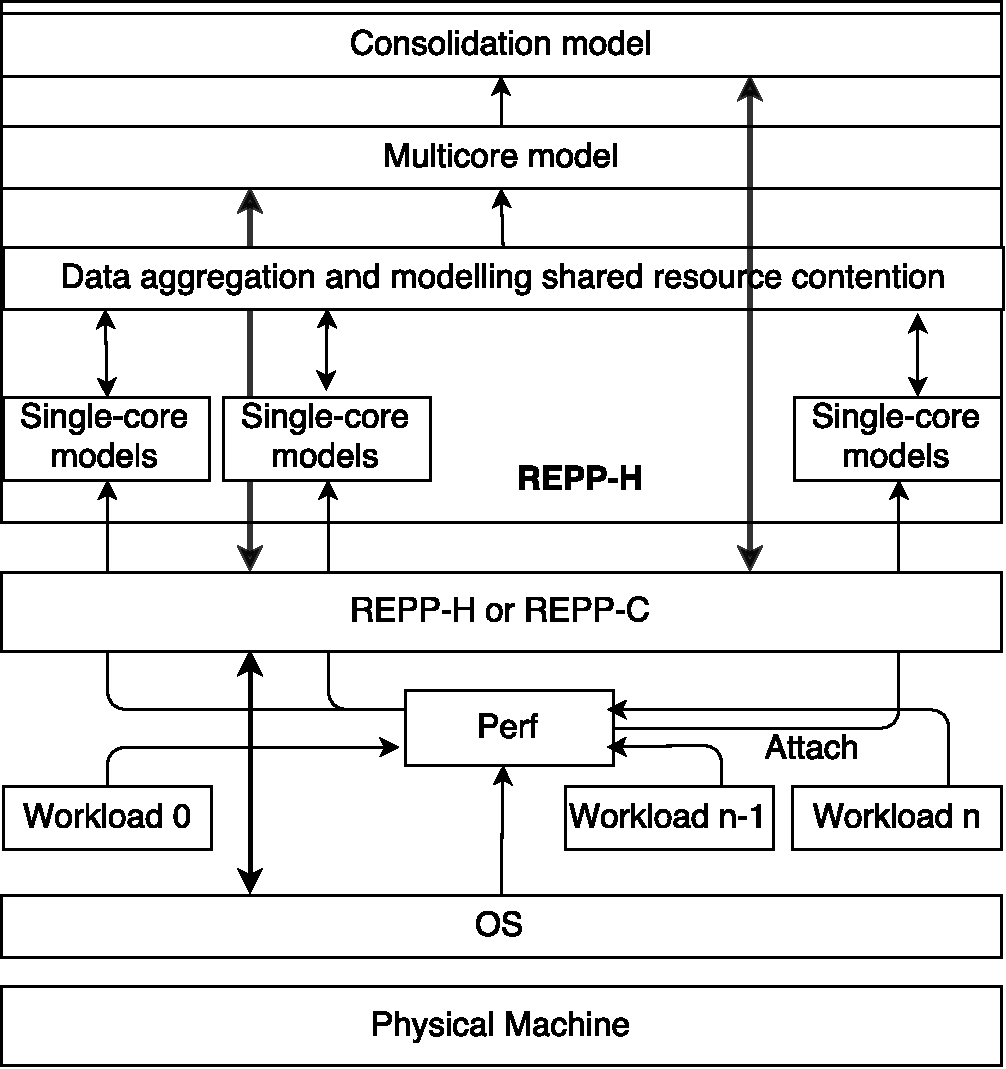
\includegraphics[width=0.8\textwidth]{Appendix1/Figs/REPP-all.pdf}
    \caption{Block diagram of REPP}
    \label{fig: reppall}
\end{figure}
\fi

In figure~\ref{fig: archrepp} shows the block diagram of REPP-H. REPP-H is attached to a
performance monitoring tool like \textsf{perf} to gather hardware counters at a period
determined empirically. The hardware monitoring counters are fed to the single core models
to predict performance and power, as the name suggests, for a single core. Next, the
results from these single core models are aggregated to predict the multicore performance
and power.  However, these single core models do not account for the contention of shared
resources.  Therefore, the results obtained from each of these single core models is added
with a correction factor determined by the contention model.  Next, to predict with core
consolidation, we introduced a scheduling technique to tackle with the impact of
intra-core and inter-core contention; thereafter, we model the impact of consolidation
only for those workloads which are collocated as a result of consolidation. Eventually,
after the prediction REPP-H and REPP-C are computed, we decide which configuration to
select based on certain set of rules. 



%Thereafter, to predict in scenarios for certain criteria, as defined by the user, can not
%be met without core consolidation; we introduce the impact of consolidation on those
%workloads are collocated due to core consolidation. Finally, after the prediction from
%both the multicore model (REPP-H), and consolidation model (REPP-C) are computed, we
%decide which configuration to select based on certain set of rules. 

%In the remainder of this appendix, we detail the implementation perspective of REPP-H
%using pseudocode. 

The power and performance estimation and control technique for a single threaded and
multiprogrammed workload (REPP-H) is defined in Algorithm~\ref{pseudo:multi}.  Given a
user-defined power or performance constraint per core ($\omega$, line~2-3), the
function~\textsl{REPP-H} is invoked periodically to satisfy the constraint. The initial
thread mapping is carried out by the Linux scheduler, which allocates threads-to-cores
such that workloads are balanced among available cores in the system~\citep{LinuxKernel}.
After a reassignment interval, we allow REPP to characterise the thread behaviour by
gathering enough performance statistics to compute the activity ratio (Table~\ref{tab:
tableactivity}) for the following components: integer unit, floating point unit, branch
prediction unit, front end, L1, L2, L3 caches, and the memory (line~4).  Thereafter, we
predict performance (section~\ref{subsec: model performance}) and power
(section~\ref{subsec: model power}) on each core at each DVFS state and Cl-State available
(lines~5-10). Since the single core predictions do not account for shared resource
contention, the total power consumed will be higher, and performance lower.  Therefore,
the modelled correction factor for power and performance is added and subtracted,
respectively, for each every prediction on a per core level (lines~11-15).
\textsl{REPP-H} returns performance and power prediction at each DVFS state and Cl-State
available (line~17).

\nomenclature[g-upsilon]{$\Upsilon$}{Potential inactive or consolidated core}

\begin{algorithm}[t]
    \caption{REPP-H}
  \label{pseudo:multi}
    \begin{algorithmic}[1]
      \Statex \Comment{Single core algorithm}
        \Function{REPP-H}{} %\funclabel{alg:multi} \label{alg:multi-line}
        \State Let $\chi(\kappa)$ be the user-defined power or performance constraint for time $T$
        \State Let $\omega$ $=$ ($\omega_{\mathit{0}}$ \ldots $\omega_{\mathit{\mathcal S-1}}$, $\omega_{\mathit{\mathcal S}}$) be distribution of $\chi(\kappa)$ for cores (0 \ldots $\mathcal S-1$, $\mathcal S$)
      \State Gather PMCs (Table~\ref{tab: tableactivity}) %\Comment{Sampling interval: \SI{250}{\milli\second}}
      \State Let {\small $REPP-H\_Pow(n, DVFS, Cl)$} be power prediction at DVFS and Cl-States per core 
      \Statex \Comment{n is core ID}
      \State Let {\small $REPP-H\_Perf(n, DVFS, Cl)$} be perf. prediction at DVFS and Cl-States per core
      \State Predict power at current configuration (Eq~\ref{eq: Predict Power})
      \State Gather PMCs at current configuration \Comment{IPS}
      \State Predict power and performance at $Cl_{\mathit{c}}$ and $P_{\mathit{f}}$ (Eq~\ref{eq: Predict Power},~\ref{eq: predictperformnceacrossp-state})
      \State Predict power and performance at $P_{\mathit{c}}$ and $Cl_{\mathit{f}}$ (Eq~\ref{eq: predictpoweracrosscl-state},~\ref{eq: predictperformnceacrosscl-state})
      \Statex \Comment{Shared resource contention}

    \ForEach{\texttt{$n \in \mathcal S$}} \Comment{$\mathcal S$ is the total number of cores}
         \ForEach{\texttt{$P_{\mathit{c}} \in $DVFS State}}
            \ForEach{\texttt{$Cl_{\mathit{c}} \in $ Cl-State}}
                \State REPP-H\_Pow(n, DVFS, Cl) = REPP\_Pow(n, DVFS, Cl) + (Eq~\ref{eq: critical error})
                \State REPP-H\_Perf(n, DVFS, Cl) = REPP\_Perf(n, DVFS, Cl) - (Eq~\ref{eq: critical error})
              \EndFor 
          \EndFor
      \EndFor
      \State \textbf{return} $REPP$-$H\_Pow$, $REPP$-$H\_Perf$
\EndFunction
    
  \end{algorithmic}
\end{algorithm}

Next, we extend the \muc power and performance prediction technique to include core
consolidation and is defined in algorithm~\ref{pseudo:models} and
algorithm~\ref{alg:algopseudo}.  With the introduction of core consolidation, the research
question to answer is -- where to allocate the thread running on the consolidated core?;
and which core to consolidate?  The core with the highest number of cache misses is chosen
as the potential inactive core ($\Upsilon$, line~4). To map threads from the inactive core
to the available cores, we introduce FACTS (Section~\ref{subsec: FACTS algo},
Algorithm~\ref{alg:algopseudo}). The thread scheduling determined by FACTS is based on the
workloads cache intensity (LLC misses) and the core's DVFS state to improve energy
efficiency. In algorithm~\ref{alg:algopseudo}, function~\textsl{FACTS} first sorts threads
in the descending order of the LLC misses (line~6) and active cores in the descending
order of the current DVFS state (line~7).  Thereafter, it allocates threads-to-cores such
that threads with highest memory bandwidth requirement are allocated to cores with lowest
DVFS state (lines~8-10). The remaining threads, if any, are allocated in the reverse order to
cores with the descending order high DVFS state and low cache misses (line~11-15).
Thereafter, in algorithm~\ref{pseudo:models}, we apply the correction factor only to
collocated threads as they have a negative performance and power impact (lines~6-10). 


\begin{algorithm}[t!]
    \caption{Prediction with REPP-H and REPP-C}
    \label{pseudo:models}
    \begin{algorithmic}[1]
        \State $REPP-H\_Pow$, $REPP-H\_Perf$ = \Call{\textsf{REPP-H}}{} \Comment{Algorithm~\ref{pseudo:multi}}
        \State Let {\small $REPP-C\_Pow(n, DVFS, Cl)$} be power prediction with consolidation
        \State Let {\small $REPP-C\_Perf(n, DVFS, Cl)$} be perf. prediction with consolidation
        \State Let $\Upsilon$ be potential inactive core \Comment{Core with highest LLC misses}
        \State TID, COREID, COREID\_C = \Call{\textsf{FACTS}}{$\Upsilon$} \Comment{Algorithm~\ref{alg:algopseudo}} 
        \ForEach{\texttt{$COREID\_C \in \mathcal S$}} 
             \ForEach{\texttt{$P_{\mathit{c}} \in $ DVFS state}}
                \ForEach{\texttt{$Cl_{\mathit{c}} \in $ Cl-State}}
                    \State REPP-C\_Pow($n_{c}$, DVFS, Cl)  = REPP-H\_Pow($n_{c}$, DVFS, Cl)  - (Eq~\ref{eq: consolidation})
                    \State REPP-C\_Perf($n_{c}$,DVFS,Cl) = REPP-H\_Perf($n_{c}$,DVFS,Cl) - (Eq~\ref{eq: consolidation})
                  \EndFor 
              \EndFor
          \EndFor
        \State DVFS state, Cl-State = \Call{\textsf{Decision}}{} \Comment{Algorithm~\ref{pseudo:conditions}}
        \State Set DVFS state, Cl-State per core 
    \end{algorithmic}
\end{algorithm}

%uses the correction factor for core consolidation and the result obtained from \textsl{REPP-H} to predict with core consolidation. 
%Algorithm~\ref{pseudo:models} defines performance and power prediction with the correction model for core consolidation. 

%Given the performance or power predictions obtained from~\textsl{REPP},
%algorithm~\ref{pseudo:models} predicts performance and power with core consolidation. The
%core with the highest number of cache misses is chosen as (potential) inactive or
%consolidated cores  

Consequent to predicting performance and power without (REPP-H) and with consolidation
(REPP-C), we introduce an algorithm (\textsl{SELCTCONFIG},
algorithm~\ref{pseudo:constraints}) to select a configuration per core such that the per
core constraint ($\omega$).  The algorithm presented is as follows: First we carry out a
linear search to find the DVFS state per core to satisfy the per core constraint (line~2).
Thereafter, we select the Cl-State, for a given DVFS state, that satisfies the constraint
(line~3); this determines the potential configuration (line~4) for performance and power
($\varpi_{\mathit{f}}$). The aforementioned process is repeated once for each algorithm,
REPP-H and REPP-C.

%\rnline{explain the figure a bit more}
%, and Figure~\ref{fig: blockrepporreppc}).  

The configuration, either REPP-H or REPP-C, is selected based on two conditions
(Algorithm~\ref{pseudo:conditions} and Section~\ref{subsec: repporreppc})
First (Condition 1, \textsf{C1}), compute the
difference between the total predicted performance and power and the performance and power
constraint (lines~4-5); second (condition 2, \textsf{C2}), compute the difference between
per thread performance and power prediction and performance and power constraint
(lines~6-8). Thereafter, check if \textsf{C1}, and \textsf{C2} are (approximately) zero
for both REPP-H and REPP-C, then select the configuration as given by REPP-H (lines~9-10).
This is because, REPP-H delivers a higher energy efficiency than REPP-C. If the constraint
is met (approximately) with \textsf{C1} for REPP-H, but \textsf{C2} for REPP-C, or
otherwise (line~12). Then, select a configuration from either REPP-C or REPP-H for which
the \textsf{C2} has lesser error (lines~13-17). Finally, select DVFS state, Cl-State per core
as given by REPP-H/REPP-C (line~12 of algorithm~\ref{pseudo:models}).

\begin{algorithm}[h!]
\caption{FACTS for K threads}
\label{alg:algopseudo}
\begin{algorithmic}[1]
\Function{FACTS}{$\Upsilon$} %\funclabel{alg:a} \label{alg:a-line}
    \While{n \textless ($\mathcal S - \Upsilon)$} \Comment{Where $\mathcal S$ is total number of cores and n $\in \mathcal S$}
        \State{Read the DVFS state}
        \ForAll{threads mapped to that core}
            \State \text{Read performance counter} \Comment{LLCM}
        \EndFor
    \EndWhile
    \State \text{Sort threads in descending order of cache misses} \Comment{LLCM array}
    \State \text{Sort cores in the descending order of DVFS state} \Comment{COREID array}
    \State \text{Let COREID\_C[] be cores with collocation}
    \While{n \textless ($\mathcal S - \Upsilon$) } 
        \State \text{Assign thread with LLCM[n] to core with COREID[n]}
    \EndWhile
    \State \text{Set a = 0, c = 0;}
    \ForAll{thread not assigned to any core} \Comment{that is, (K \textgreater $\mathcal S - \Upsilon$)}
        \State \text{Assign thread with LLCM[$\mathcal S - \Upsilon$-c] to core with COREID[a]} 
        \State \text{COREID\_C[a] = COREID[a]}
        \State \text{a = a+1; c = c+1;}
    \EndFor
    \State \textbf{return} $LLCM, COREID, COREID\_C$
\EndFunction
\end{algorithmic}
\end{algorithm}

\begin{algorithm}[h!]
    \caption{REPP-H and REPP-C Select configuration}
    \label{pseudo:constraints}
  \begin{algorithmic}[1]
      \Function{SelectConfig}{$\omega$, $Pow$, $Perf$} %\funclabel{alg:a1} \label{alg:a-line1}
          \State Perform a linear search on $Pow$ and $Perf$ to determine the nearest $\omega$ per core
          \State Select Cl-State for the given DVFS State that satisfies $\omega$ per core.
          \State Configuration $\alpha_{\mathit{f}}$ is DVFS, Cl-State
          \State \textbf{return} $\rho_{\mathit{f}}$, $\eta_{\mathit{f}}$
      \EndFunction
  \end{algorithmic}
\end{algorithm}



\nomenclature[g-varpi]{$\varpi_{\mathit{f}}$}{Future configuration for predicted performance and power to satisfy $\omega$}
\begin{algorithm}[h!]
    \caption{Selecting REPP-H or REPP-C}
    \label{pseudo:conditions}
  \begin{algorithmic}[1]
      \Function{Decision}{}
        \State {\small REPP-H($\varpi_{\mathit{f}}$)}[n] = \Call{\textsf{SelectConfig}}{$\omega$, {\small $REPP$-$H\_Pow$, $REPP$-$H\_Perf$}} 
        \Statex \Comment{$\varpi_{\mathit{f}}$ = ($\rho_{\mathit{f}}$, $\eta_{\mathit{f}}$) for $\omega$}
        \State {\small REPP-C($\varpi_{\mathit{f}}$)}[n]= \Call{\textsf{SelectConfig}}{$\omega$, {\small $REPP$-$C\_Pow$, $REPP$-$C\_Perf$}} 
        \Statex \Comment{n is the thread ID}
        %\State Select REPP-H or REPP-C (Algorithm~\ref{pseudo:conditions})
        
        %\State $REPP-H(\varpi_{\mathit{f}})[n]$       \Comment{n is the thread ID}
        %\State $REPP-C(\varpi_{\mathit{f}})[n]$
        \vspace{1mm}
        \State $REPP_{C1}[n] = (\omega - \sum_{n=0}^{n=\mathcal S} REPP(\varpi_{\mathit{f}}))$
        \State $REPP-C_{C1}[n] = (\omega - \sum_{n=0}^{n=\mathcal S} REPP-C(\varpi_{\mathit{f}}))$
        \ForEach {$n \in \mathcal S $} 
            \State $REPP_{C2}[n]   = (\omega_{n} - REPP(\varpi_{\mathit{f}})[n])$
            \State $REPP-C_{C2}[n]   = (\omega_{n} - REPP-C(\varpi_{\mathit{f}})[n])$
        \EndFor
        \If{$REPP_{C1}\apeq REPP-C_{C1} \apeq REPP_{C2} \apeq REPP-C_{C2} \apeq 0$}
            \State \textbf{return} REPP[n]% \Comment{REPP has better throughput-per-watt}
        \ElsIf{\\
            ($REPP_{C1} \apeq 0 $ \textsf{and} $\sum_{n=0}^{n=\mathcal S}REPP-C_{C2}[n] \apeq 0$) \textsf{or} ($\sum_{n=0}^{n=\mathcal S} REPP_{C2}[n] \apeq 0 $ \textsf{and} $REPP-C_{C1} \apeq 0 $)}
            \If{$\sum_{n=0}^{n=\mathcal S}REPP_{C2}[n]$ > $\sum_{n=0}^{n=\mathcal S}REPP-C_{C2}[n]$}
            \State Allocate threads-to-cores as given by FACTS
            \State \textbf{return} REPP-C
            \Else
            \State \textbf{return} REPP-H
            \EndIf
        \EndIf
    \EndFunction
  \end{algorithmic}
\end{algorithm}

\iffalse
\begin{figure}[h]
    \hspace{4em}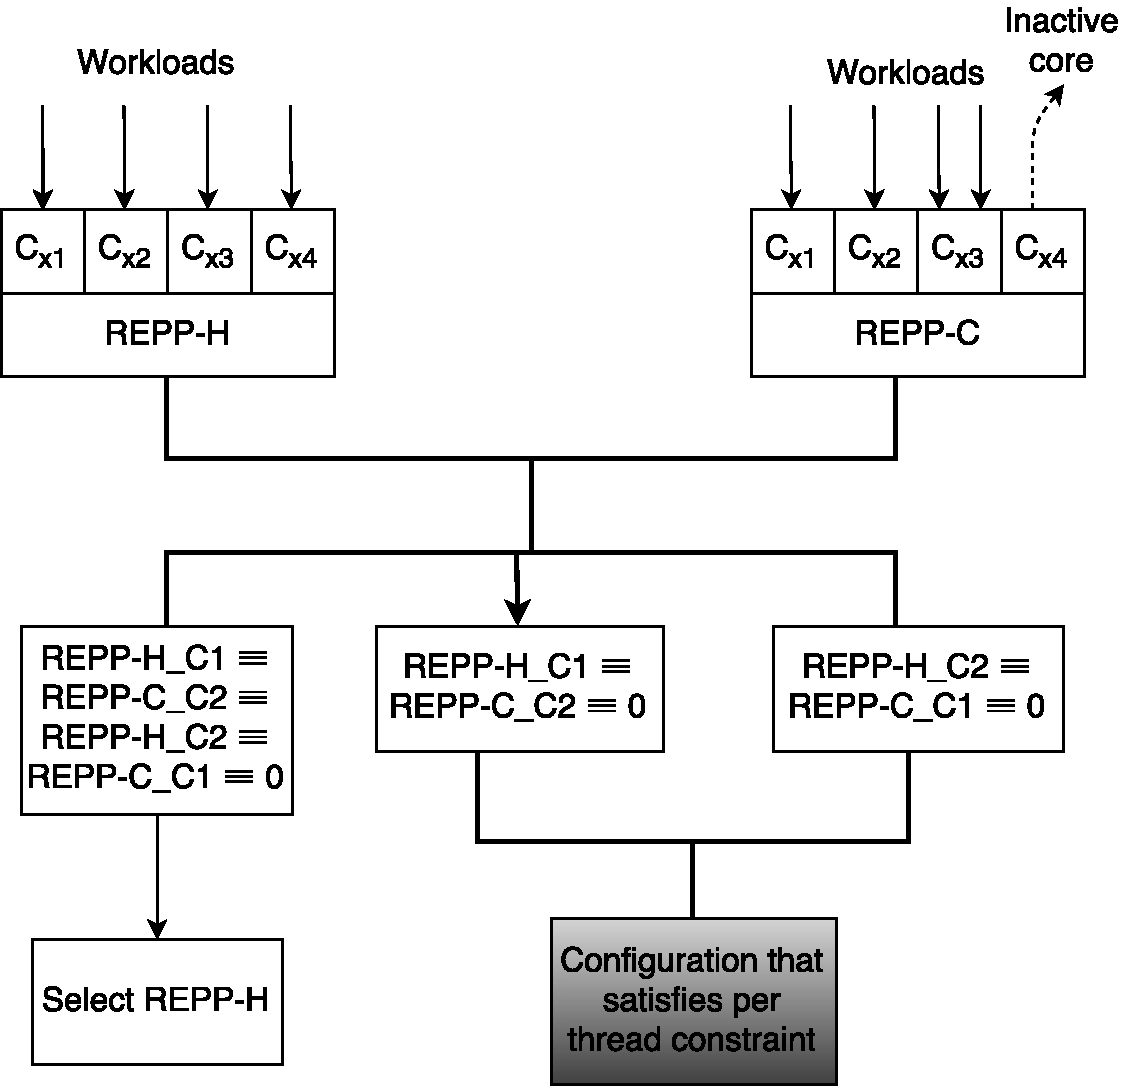
\includegraphics[width=0.8\textwidth]{Appendix1/Figs/repporreppc.pdf}
    \caption[Selecting REPP-H or REPP-C]{\captitle{Selecting REPP-H or REPP-C} Block diagram illustration of algorithm~\ref{pseudo:conditions}. Conditions \textsf{C1} and \textsf{C2} determine whether the system is meeting the system performance and power constraint or per thread performance and power, respectively.}
    \label{fig: blockrepporreppc}
\end{figure}
\fi

